\documentclass[12pt]{article}
\usepackage{graphicx}
\usepackage{amsmath, amssymb, amsthm}
\usepackage{geometry}
\geometry{margin=1in}

\title{Personal Assignment 2}
\author{Mubarak}
\date{}

\begin{document}

\maketitle

\section*{1. Cari semua turunan parsial kedua}

\subsection*{(a) $f(x,y)=x^4 y - 2x^3 y^2$}

Hitung turunan pertama dulu:
\[
\begin{aligned}
f_x(x,y)&=\frac{\partial}{\partial x}\big(x^4 y - 2x^3 y^2\big)
=4x^3 y - 6x^2 y^2,\\[6pt]
f_y(x,y)&=\frac{\partial}{\partial y}\big(x^4 y - 2x^3 y^2\big)
=x^4 - 4x^3 y.
\end{aligned}
\]

Sekarang turunan kedua:
\[
\begin{aligned}
f_{xx}(x,y)&=\frac{\partial}{\partial x}(4x^3 y - 6x^2 y^2)
=12x^2 y - 12x y^2 = 12xy(x-y),\\[6pt]
f_{yy}(x,y)&=\frac{\partial}{\partial y}(x^4 - 4x^3 y)
=-4x^3,\\[6pt]
f_{xy}(x,y)&=\frac{\partial}{\partial y}(4x^3 y - 6x^2 y^2)
=4x^3 - 12x^2 y = 4x^2(x-3y),\\[6pt]
f_{yx}(x,y)&=\frac{\partial}{\partial x}(x^4 - 4x^3 y)
=4x^3 - 12x^2 y = 4x^2(x-3y).
\end{aligned}
\]
(Terlihat $f_{xy}=f_{yx}$ seperti diharapkan.)

\subsection*{(b) $z=\dfrac{y}{2x+3y}$}

Definisikan $D=2x+3y$. Dengan aturan pembagian (quotient rule) untuk turunan parsial:

\subsubsection*{Turunan pertama}
\[
\begin{aligned}
z_x &= \frac{0\cdot D - y\cdot(2)}{D^2} = -\frac{2y}{(2x+3y)^2}, \\[6pt]
z_y &= \frac{1\cdot D - y\cdot(3)}{D^2}
= \frac{2x+3y-3y}{(2x+3y)^2}
= \frac{2x}{(2x+3y)^2}.
\end{aligned}
\]

\subsubsection*{Turunan kedua}
Turunan $z_x$ terhadap $x$:
\[
\begin{aligned}
z_{xx}
&= \frac{\partial}{\partial x}\Big(-2y(2x+3y)^{-2}\Big) \\
&= -2y \cdot (-2)(2x+3y)^{-3} \cdot 2 \\
&= 8y(2x+3y)^{-3} \\
&\Rightarrow\quad z_{xx} = \frac{8y}{(2x+3y)^3}.
\end{aligned}
\]

Turunan $z_y$ terhadap $y$:
\[
\begin{aligned}
z_{yy}
&= \frac{\partial}{\partial y}\Big(2x(2x+3y)^{-2}\Big) \\
&= 2x \cdot (-2)(2x+3y)^{-3} \cdot 3 \\
&= -12x(2x+3y)^{-3} \\
&\Rightarrow\quad z_{yy} = \frac{-12x}{(2x+3y)^3}.
\end{aligned}
\]

Turunan silang (contoh $z_{xy}$, lalu $z_{yx}$ untuk verifikasi):
\[
\begin{aligned}
z_{xy}
&= \frac{\partial}{\partial y}\Big(-2y(2x+3y)^{-2}\Big) \\
&= -2(2x+3y)^{-2} + (-2y)\cdot(-2)(2x+3y)^{-3}\cdot 3 \\
&= -\frac{2}{(2x+3y)^2} + \frac{12y}{(2x+3y)^3} \\
&= \frac{-4x + 6y}{(2x+3y)^3}.
\end{aligned}
\]

Jika dihitung $z_{yx} = \partial_x(z_y)$ diperoleh hasil yang sama:
\[
z_{yx}=\frac{-4x+6y}{(2x+3y)^3}.
\]

Jadi ringkasan turunan kedua untuk (b):
\[
\boxed{z_{xx}=\dfrac{8y}{(2x+3y)^3},\quad
z_{yy}=\dfrac{-12x}{(2x+3y)^3},\quad
z_{xy}=z_{yx}=\dfrac{-4x+6y}{(2x+3y)^3}}.
\]

\section*{2. Jelaskan $\mathbf{F}$ dan buat sketsa beberapa vektor dalam medan vektor $\mathbf{F}(x,y)$}

\subsection*{(a) $\displaystyle \mathbf{F}(x,y)=x\,\mathbf{i}+\tfrac{1}{2}y\,\mathbf{j}$}

\textbf{Interpretasi.} Pada titik $(x,y)$ vektornya adalah $(M,N)=(x,\tfrac12 y)$.

\item Komponen-$x$ sebanding dengan $x$. Jika $x>0$ arah ke kanan, jika $x<0$ ke kiri.
    \item Komponen-$y$ sebanding dengan $y$ tetapi setengah besarannya.
    \item Divergensi: $\nabla\cdot\mathbf{F}=\partial_x(x)+\partial_y(\tfrac12 y)=1+\tfrac12=\tfrac32>0$ → medan ``menyebar'' (sumber).
    \item Titik asal $(0,0)$ adalah titik nol vektor.

Beberapa vektor contoh dapat digambarkan berdasarkan koordinat dan komponen.


\begin{array}{c|c}
\text{Titik }(x,y) & \mathbf{F}(x,y) = \left(x, \tfrac{1}{2} y\right) \\ \hline
(0,0) & (0,0) \\
(1,0) & (1,0) \\
(0,1) & \left(0,\tfrac{1}{2}\right) \\
(1,1) & \left(1,\tfrac{1}{2}\right) \\
(-1,1) & \left(-1,\tfrac{1}{2}\right) \\
(2,0) & (2,0)
\end{array}

\begin{figure}[htbp]
    \centering
    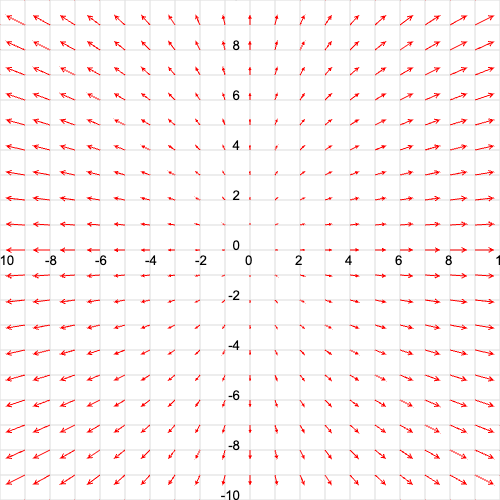
\includegraphics[width=0.6\textwidth]{personal_assignment_2_2_a.png}
    \caption{Vector Field}
    \label{fig:my_label_1}
\end{figure}

\subsection*{(b) $\displaystyle \mathbf{F}(x,y)=y\,\mathbf{i}+(x+y)\,\mathbf{j}$}

\textbf{Interpretasi.} Pada titik $(x,y)$ vektornya $(M,N)=(y,x+y)$.

\item Komponen-$x$ bergantung pada $y$, komponen-$y$ bergantung pada $x$ dan $y$.
    \item Divergensi: $\nabla\cdot\mathbf{F}=\partial_x (y)+\partial_y(x+y)=0+1=1>0$.
    \item Periksa rotasi (curl) 2D: $\mathrm{curl}_z=\partial_x N - \partial_y M = \partial_x(x+y)-\partial_y(y)=1-1=0$. Karena curl = 0 di $\mathbb{R}^2$ (domain sederhana), medan ini konservatif — ada potensial skalar.
    
    Potensial $\phi(x,y)$ dapat dicari: dari $\phi_x = y \Rightarrow \phi(x,y)=xy + g(y)$. Dari $\phi_y = x + g'(y)$ harus sama dengan $x+y \Rightarrow g'(y)=y \Rightarrow g(y)=\tfrac{1}{2}y^2$. Jadi
    \[
    \phi(x,y)=xy+\tfrac{1}{2}y^2 + C.
    \]

Beberapa vektor contoh dapat digambarkan berdasarkan koordinat dan komponen.


\begin{array}{c|c}
(x,y) & \mathbf{F}(x,y) = (y,\, x+y) \\ \hline
(0,0) & (0,0) \\
(1,0) & (0,1) \\
(0,1) & (1,1) \\
(1,1) & (1,2) \\
(-1,1) & (1,0) \\
(2,-1) & (-1,1)
\end{array}

\begin{figure}[htbp]
    \centering
    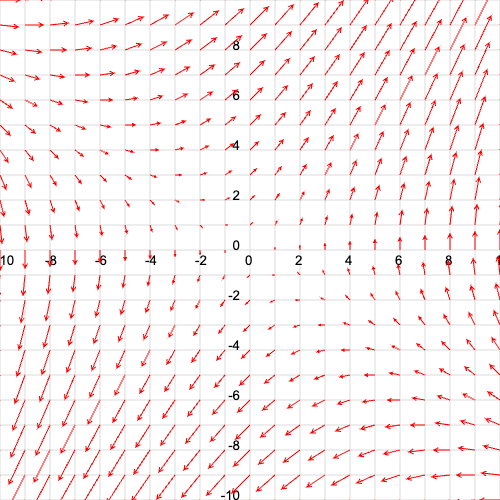
\includegraphics[width=0.6\textwidth]{personal_assignment_2_2_b.png}
    \caption{Vector Field}
    \label{fig:my_label_2}
\end{figure}


\section*{3. Gunakan Cramer’s Rule untuk menyelesaikan sistem (LO2)}

Sistem:
\[
\begin{cases}
2x_1 + x_2 - x_3 = 2,\\[4pt]
5x_1 + 2x_2 -2x_3 = 9,\\[4pt]
3x_1 + x_2 + x_3 = 5.
\end{cases}
\]

Tuliskan matriks koefisien $A$ dan vektor ruas kanan $b$:
\[
A = \begin{pmatrix}
2 & 1 & -1 \\
5 & 2 & -2 \\
3 & 1 & 1
\end{pmatrix}, \qquad
b = \begin{pmatrix}
2 \\
9 \\
5
\end{pmatrix}.
\]

\subsubsection*{Determinan $\det(A)$}
Menghitung determinan $A$ (metode Sarrus atau ekspansi):
\[
\det(A) = -2.
\]
(Penghitungan singkat: $2\cdot2\cdot1 + 1\cdot(-2)\cdot3 + (-1)\cdot5\cdot1 -\big((-1)\cdot2\cdot3 + 1\cdot5\cdot1 + 2\cdot(-2)\cdot1\big) = -2$.)

Karena $\det(A)\neq 0$, solusi unik ada.

\subsubsection*{Matriks $A_1,A_2,A_3$ (mengganti kolom sesuai variabel)}

\item $A_1 = A$ dengan kolom ke-1 diganti $b$:
    \[
    A_1 = \begin{pmatrix}
    2 & 1 & -1 \\
    9 & 2 & -2 \\
    5 & 1 & 1
    \end{pmatrix},
    \qquad \det(A_1) = -10.
    \]

    \item $A_2 = A$ dengan kolom ke-2 diganti $b$:
    \[
    A_2 = \begin{pmatrix}
    2 & 2 & -1 \\
    5 & 9 & -2 \\
    3 & 5 & 1
    \end{pmatrix},
    \qquad \det(A_2) = 18.
    \]

    \item $A_3 = A$ dengan kolom ke-3 diganti $b$:
    \[
    A_3 = \begin{pmatrix}
    2 & 1 & 2 \\
    5 & 2 & 9 \\
    3 & 1 & 5
    \end{pmatrix},
    \qquad \det(A_3) = 2.
    \]

\subsubsection*{Solusi menurut Cramer}
\[
x_1=\frac{\det(A_1)}{\det(A)}=\frac{-10}{-2}=5,\qquad
x_2=\frac{\det(A_2)}{\det(A)}=\frac{18}{-2}=-9,\qquad
x_3=\frac{\det(A_3)}{\det(A)}=\frac{2}{-2}=-1.
\]

\textbf{Jadi solusi:} $\boxed{x_1=5,\; x_2=-9,\; x_3=-1}$.

\section*{4. Gunakan Gauss–Jordan untuk menyelesaikan (LO2)}

Mulai dari matriks augmentasi $[A|b]$:
\[
\left[\begin{array}{ccc|c}
2 & 1 & -1 & 2 \\[4pt]
5 & 2 & -2 & 9 \\[4pt]
3 & 1 & 1 & 5
\end{array}\right]
\]

\textbf{Langkah 1.} Bagi baris 1 dengan 2 agar pivot = 1:
\[
R_1 \leftarrow \tfrac{1}{2}R_1
\quad\Rightarrow\quad
\left[\begin{array}{ccc|c}
1 & \tfrac{1}{2} & -\tfrac{1}{2} & 1 \\[4pt]
5 & 2 & -2 & 9 \\[4pt]
3 & 1 & 1 & 5
\end{array}\right]
\]

\textbf{Langkah 2.} Hapus elemen bawah di kolom 1:
\[
\begin{aligned}
R_2 &\leftarrow R_2 - 5R_1,\\
R_3 &\leftarrow R_3 - 3R_1.
\end{aligned}
\]
Hasil:
\[
\left[\begin{array}{ccc|c}
1 & \tfrac{1}{2} & -\tfrac{1}{2} & 1 \\[4pt]
0 & -\tfrac{1}{2} & \tfrac{1}{2} & 4 \\[4pt]
0 & -\tfrac{1}{2} & \tfrac{5}{2} & 2
\end{array}\right]
\]

\textbf{Langkah 3.} Buat pivot 1 pada baris 2: kalikan $R_2$ dengan $(-2)$:
\[
R_2 \leftarrow -2R_2
\quad\Rightarrow\quad
\left[\begin{array}{ccc|c}
1 & \tfrac{1}{2} & -\tfrac{1}{2} & 1 \\[4pt]
0 & 1 & -1 & -8 \\[4pt]
0 & -\tfrac{1}{2} & \tfrac{5}{2} & 2
\end{array}\right]
\]

\textbf{Langkah 4.} Hilangkan entri kolom 2 pada baris 1 dan baris 3:
\[
\begin{aligned}
R_1 &\leftarrow R_1 - \tfrac{1}{2} R_2,\\
R_3 &\leftarrow R_3 + \tfrac{1}{2} R_2.
\end{aligned}
\]
Hasil:
\[
\left[\begin{array}{ccc|c}
1 & 0 & 0 & 5 \\[4pt]
0 & 1 & -1 & -9 \\[4pt]
0 & 0 & 2 & -2
\end{array}\right]
\]

\textbf{Langkah 5.} Bagi baris 3 dengan 2 untuk membuat pivot 1, lalu hilangkan entri kolom 3 di baris 2:
\[
R_3 \leftarrow \tfrac{1}{2}R_3 \quad\Rightarrow\quad
\left[\begin{array}{ccc|c}
1 & 0 & 0 & 5 \\[4pt]
0 & 1 & -1 & -9 \\[4pt]
0 & 0 & 1 & -1
\end{array}\right]
\]

Lalu
\[
R_2 \leftarrow R_2 + R_3
\quad\Rightarrow\quad
\left[\begin{array}{ccc|c}
1 & 0 & 0 & 5 \\[4pt]
0 & 1 & 0 & -9 \\[4pt]
0 & 0 & 1 & -1
\end{array}\right].
\]

Maka bentuk tereduksi (RREF) menunjukkan solusi langsung:
\[
x_1 = 5,\quad x_2 = -9,\quad x_3 = -1.
\]

\end{document}